\documentclass[11pt,a4paper]{report}
\usepackage[margin=0.5in]{geometry}
\usepackage[explicit]{titlesec}
\usepackage[dvipsnames]{color}
\usepackage{graphicx}
\usepackage{alltt}

\definecolor{mygray}{gray}{.75}

\titleformat{name=\section,numberless}[display]
  {\normalfont\scshape\Large}
  {\hspace*{-10pt}#1}
  {-15pt}
  {\hspace*{-110pt}\rule{\dimexpr\textwidth+80pt\relax}{2pt}\Huge}
\titlespacing*{\section}{0pt}{30pt}{10pt}

\titleformat{name=\subsection,numberless}[display]
  {\normalfont\scshape}
  {\hspace*{-10pt}#1}
  {-15pt}
  {\hspace*{-110pt}\rule{\dimexpr\textwidth+30pt\relax}{0.4pt}\Huge}
\titlespacing*{\subsection}{0pt}{20pt}{5pt}


\begin{document}

\noindent\Large\textbf{CM2303 (Algorithms \& Data Structures)}\\
\noindent\large\textit{Non-assessed Labs}
\vskip30pt

\section*{Lab 2.6: Greedy Algorithms}

A greedy algorithm is a heuristic that tries to find the best solution to a problem by making the \textit{next best} decision at each stage. In some cases, it is rare that a greedy algorithm will find the most optimal solution, but the algorithmic complexity is much smaller. In this exercise, we will use greedy algorithms to solve two different types of problem.

Lab 2.6 requires your \texttt{Stack} implementation from Lab 2.3, but otherwise has no prerequisite labs.

\begin{enumerate}

\item The \textit{coin change problem} involves an attempt to reach a target sum of money using the smallest number of coins of a particular denomination. For example, consider the current set of coins in circulation in the UK (in percentage of pound sterling):
    \begin{center}
       1, 2, 5, 10, 20, 50, 100, 200
    \end{center}

    A greedy algorithm tasked with finding the smallest number of coins in a given target would, at each stage, use the largest coin available before the target sum is reached. Therefore, to reach \pounds2.74, the algorithm would use the coins:
    \begin{center}
        200, 50, 20, 2, 2
    \end{center}

    Write a method for solving the coin-change problem using a greedy algorithm that accepts two arguments: an integer array (representing the set of coins available to use) and an integer target. The method should return a list of coins used. The below pseudocode illustrates one method you might use to accomplish this.

\begin{alltt}
Procedure greedy\_coin\_change:
    Inputs: \(coins\) (integer array), \(target\) (integer)
    Output: \(coins\_used\) list/array of coins used
    
    \(coins \gets coins\) sorted in descending order
    \(coins\_used \gets\) empty list of integers
    while \(target > 0\):
        if \(\exists coin \in coins \leq target\):
            \(largest\_coin \gets\) largest coin value \(\leq target\)
            \(coins \gets coins + \{largest\_coin\}\)
            \(target \gets target - largest\_coin\)
        else:
            break
    return \(coins\_used\)
\end{alltt}

\item Verify that your function works by passing it the pound sterling coin set and checking that the coins used to form \pounds2.74 match those used in the example in the previous question. (\textit{Hint: to check, simply iterate over the list of coins used and print them out}).
        
\item The pound sterling coin set contains a one-pence piece, which means that a greedy algorithm will \textit{always} find an optimal solution for valid GBP sums of money. Now consider the following coin set:
    \begin{center}
        100, 25, 10, 4
    \end{center}
    It is possible to form the sum of 241 arbitrary units by using these coins:
    \begin{center}
        100, 100, 25, 4, 4, 4, 4
    \end{center} 
    
    Pass this coin set and target value to your greedy algorithm and print out the resultant list of coins used. Does the method manage to find an optimal solution? 

    If your greedy algorithm is implemented correctly, the algorithm will instead make up the sum of 239. Whilst this is close to the target, it is not the closest possible given the coins available. As such, the greedy algorithm has found a \textit{local optimum} based on the decisions it makes to always choose the largest coin possible. The \textit{global optimum} in this case is equal to the exact 241 solution required, but a more intelligent (and probably more complex) algorithm would be required to reach this global optimum.

\item The travelling salesman problem (TSP) is famous in computer science and there are a number of methods that can be employed to try and find optimal solutions. A greedy algorithm can be used to find a local optimum solution for the TSP.

    The TSP is focussed around a salesperson, who must travel to a set of cities to buy/sell goods. The cities exist on a weighted graph, where the respective edge weightings refer to the distances between cities. The algorithm starts at one city and, at each stage, chooses the closest city from the current city that hasn't yet been visited.

    \begin{center}
    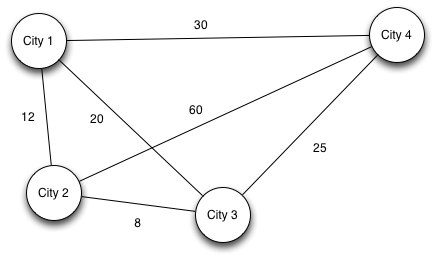
\includegraphics[width=.6\textwidth]{media/tsp1.png}
    \end{center}

    In the above example, the algorithm, starting from City 1, will first choose to travel to City 2, then City 3, and finally City 4, giving a total distance of 45.

    To implement an adjacency matrix in Java (to represent the distances between cities), a simple 2-dimensional integer array can be used, where \texttt{distances[i][j] == distances[j][i]} and is equal to the distance between cities \texttt{i} and \texttt{j}. For example, the above city graph can be represented by the following adjacency matrix (where index 0 = City 1, index 1 = City 2, etc.).

    \begin{center}\texttt{00  12  20  30 \\
        12  00  08  20 \\
        20  08  00  25 \\
        30  20  25  00}
    \end{center}

    Write a method that generates and returns a random distance matrix for a given number of cities. The method should accept three arguments: an integer number of cities to generate, a minimum allowed distance and a maximum allowed distance.

\item Write a method that attempts to solve the TSP, given a particular distance matrix. The method should return some kind of reference to the order of cities visited by the algorithm. The method should use the indices of the 2D array as city identifiers and start the journey from the first city (i.e. the one at index 0).

    An example implementation is provided below. If you choose to use this method, you could use your stack implementation from Lab 2.3 (you will need to modify it to work with Integers and to support the \texttt{peek()} method and any others you may need, if it doesn't already support them).

\begin{alltt}
Procedure greedy\_travelling\_salesman:
    Input: \(distances\) (2-dimensional integer array)
    Output: \(vitied\_cities\) (stack)

    \(visited\_cities \gets \) empty stack
    push first city onto \(visited\_cities\)

    while size of \(visited\_cities < \) number of cities:
        \(current\_city \gets\) peek at \(visited\_cities\)
        \(next\_city \gets\) city closest to \(current\_city\) that is still unvisited
        push \(next\_city\) onto \(visited\_cities\)
    
    return \(visited_cities\)
\end{alltt}

\item Use your city-generator to create an adjacency matrix of 5 cities with suitable distance range (e.g. between 1 and 30). Your procedure should print the generated matrix in a similar way to that shown in Question 4.

\item Pass the distance matrix to your greedy TSP algorithm. Look at the matrix manually to work out the route that the algorithm should take. Does this match the cities returned as $visited\_cities$ from your method? (\textit{Note: If you used a stack, as in the above implementation, then your list of cities will be ordered backwards if iterating over normally}).
    

\end{enumerate}

\end{document}
